\newpage
\section{Implementacja}		%4

\subsection{Struktura Node}

Pierwszym istotnym elementem jest struktura \texttt{Node}, która reprezentuje pojedynczy węzeł \\
w podwójnie powiązanej liście. Definicję klasy \texttt{Node} przedstawiono na listingu \textbf{2}:

\lstinputlisting[caption=Struktura Node, label={lst:listing-node.cpp}, language=C++]{kod/node.cpp}

Struktura ta definiuje trzy podstawowe atrybuty: wartość przechowywaną \\ w węźle, wskaźnik na następny węzeł oraz wskaźnik na poprzedni węzeł. Konstruktor inicjalizuje te atrybuty.

\subsection{Klasa DoublyLinkedList}

Główna klasa, \texttt{DoublyLinkedList}, zawiera metody do dodawania, usuwania oraz przeszukiwania węzłów.
Jej strukturę przedstawiono na listingu \textbf{3}

\lstinputlisting[caption=Klasa DoublyLinkedList, label={lst:listing-doubly_linked_list.cpp}, language=C++]{kod/doubly_linked_list.cpp}

\subsection{Klasa App}

Klasa App, posiadająca jedynie składowe statyczne odpowiada za uruchomnienie programu i wyświetlanie interfejsu użytkownika.
Jej strukturę przedstawiono na listingu \textbf{4}

\lstinputlisting[caption=Klasa App, label={lst:listing-app.cpp}, language=C++]{kod/app.cpp}

\subsection{Wyniki implementacji}

\subsubsection{Obsługa programu}
Na rysunku \textbf{4.1} przedstawiono menu główne programu.

\begin{figure}[!htb]
	\begin{center}
		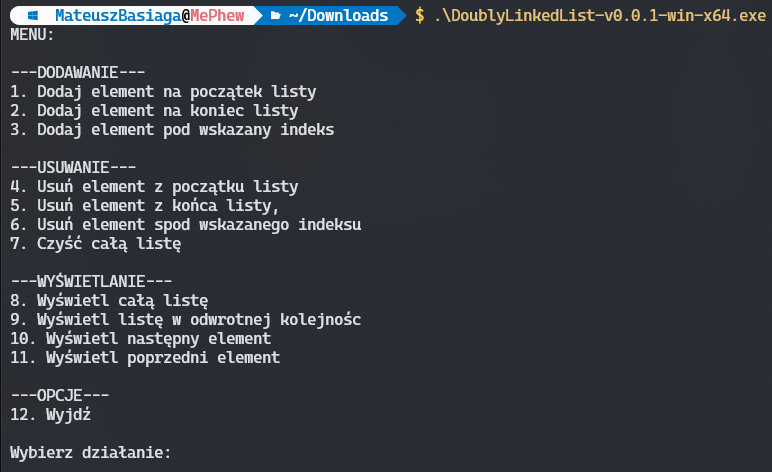
\includegraphics[width=\textwidth]{rys/menu.png}
		\caption{Menu główne programu}\label{rys:menu_programu}
	\end{center}
\end{figure}

\subsection{Wykorzystanie systemu Git i platformy GitHub}

Wdrożono automatyczną publikację nowych wersji programu w ramach systemu CI.
Na rysunku \textbf{4.2} pokazano pierwszą opublikowaną wersję programu.

\begin{figure}[!htb]
	\begin{center}
		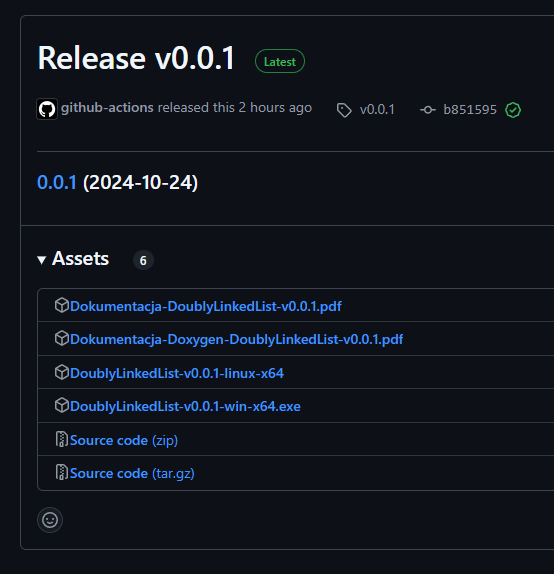
\includegraphics[width=\textwidth]{rys/ci-release.png}
		\caption{Pierwsza opublikowana wersja programu}\label{rys:ci_release}
	\end{center}
\end{figure}

Jak widać powyżej do każdej wersji programu dołączane są załączniki zawierające dokumentację kodu oraz
pliki wykonywalne na platformy Windows oraz Linux.
